\chapter{Appendix A}

\label{section:behaviour_tree_syntax}
\section{Behavior trees syntax}

In this small section we want to give a small overview of the terminology and syntax of BTs to allow reader unfamiliar with them to understand the ones presented in the remainder of the chapter.

A behavior tree is a directed tree in which the nodes are classified as root, control flow nodes, or execution nodes (tasks). Some of this nodes are represented in Figures \ref{fig:begin_bt_nodes} to \ref{fig:end_bt_nodes}.
The root of the tree (\Cref{fig:begin_bt_nodes}) is the starting point of the action plan and it’s the only node with no parent, control flow nodes are all those nodes with a single parent and one or more children and execution nodes are the leaves of the tree. 

The execution of a behavior tree starts from the root which sends ticks with a certain frequency to its child. A tick signals to a node that it can start or continue its execution. Each executing node can return to the parent either running, if couldn’t complete it’s execution with a given tick, success if it success if it has achieved its goal, or failure otherwise. 

Conventionally, nodes in a BT are placed top to bottom, left to right, so each children is placed directly below its parent and children are ordered starting from the leftmost one. In our work however we decided to follow the approach proposed by Angelouv \cite{bt_abuse}, which instead goes left to right, top to bottom.

The order of execution of the nodes in the tree is controlled by the control flow nodes (\Cref{fig:bt_control_flow_nodes}), which determine if their children must be executed, in which order and whether there are some conditions that might determine the abortion of their operation.
There are different types of control flows nodes and in our work we used the following:
\begin{description}
\item[\textbf{Selector}] A selector node (also called fallback), shown in \Cref{fig:bt_selector}, executes each of its children sequentially until one of them succeeds, in which case it returns success, otherwise it fails. It is used when different strategies can be used to achieve a given result and just one of them has to succeed for the whole task to be a success.
\item[\textbf{Sequence}] A sequence node, shown in \Cref{fig:bt_sequence}), executes each of its children sequentially until one of them fails, in which case it return failure, otherwise it succeeds. It is used to represent sequences of actions that must be performed from start to finish to be successful.
\item[\textbf{Parallel}] unlike the previous two, for a parallel task there isn’t still definition or symbol. In our trees they are represented as in shown in \Cref{fig:bt_parallel}). In our interpretation, a parallel node executes each of its children in parallel, until the first one fails, in which case the task stops all its children and returns failure. 
\end{description}

\begin{figure}[ht]
\centering

\includegraphics[height=1cm]{Images/images/bt/root.drawio.png} 
\caption{Root node.}
\label{fig:begin_bt_nodes}
\end{figure}

\begin{figure}[ht]
\centering
\begin{subfigure}[t]{3cm}
\centering
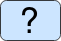
\includegraphics[height=1cm]{Images/images/bt/selector.drawio.png} 
\caption{Selector}
\label{fig:bt_selector}
\end{subfigure}
\begin{subfigure}[t]{3cm}
\centering
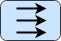
\includegraphics[height=1cm]{Images/images/bt/parallel.drawio.png} 
\caption{Parallel}
\label{fig:bt_parallel}
\end{subfigure}
\begin{subfigure}[t]{3cm}
\centering
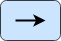
\includegraphics[height=1cm]{Images/images/bt/sequence.drawio.png} 
\caption{Sequence}
\label{fig:bt_sequence}
\end{subfigure}
\caption{Composite/Control flow nodes.}
\label{fig:bt_control_flow_nodes}
\end{figure}

\begin{figure}[ht]
\centering
\begin{subfigure}[t]{3.5cm}
\centering

\includegraphics[height=1cm]{Images/images/bt/success.drawio.png} 
\caption{Success}
\label{fig:bt_success}
\end{subfigure}
\begin{subfigure}[t]{3.5cm}
\centering

\includegraphics[height=1cm]{Images/images/bt/failure.drawio.png} 
\caption{Failure}
\label{fig:bt_failure}
\end{subfigure}
\begin{subfigure}[t]{3.5cm}
\centering
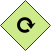
\includegraphics[height=1cm]{Images/images/bt/repeat.drawio.png} 
\caption{Repeat}
\label{fig:bt_repeat}
\end{subfigure}
\caption{Decorator nodes.}
\label{fig:bt_decorator_nodes}
\end{figure}

\begin{figure}[H]
\centering
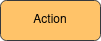
\includegraphics[height=1cm]{Images/images/bt/action.drawio.png} 
\caption{Execution node.}
\label{fig:end_bt_nodes}
\end{figure}

Some advanced implementation of BT, like the ones offered by Unreal Engine, offer another way to control the execution order of children by letting users define conditions which, when verified, lead to the abortion of the execution of a child to immediately start executing another one with with higher priority. There is no general consensus on the name of this technique, Unreal Engine defines this as Observer Abort. 

Another type of node are the \textbf{Decorator} nodes (\ref{fig:bt_decorator_nodes}. Decorator nodes, as the name suggest, "decorate" another node in the tree by altering the way it is executed or changing its return value. Examples of decorator nodes are the \textbf{Success} which executes the child, but always returns success (\Cref{fig:bt_success}), \textbf{Failure}, which executes the child, but always returns false (\Cref{fig:bt_failure}) and \textbf{Repeat}, which repeats for a given amount of time the child, unless it returns failure (\Cref{fig:bt_repeat}).

Finally, as leaves of the tree, execution nodes (\Cref{fig:end_bt_nodes}) define the possible actions that a bot can perform, like shooting a gun or moving to a specific location.

By combining control nodes, decorator nodes and execution nodes, many different and arbitrarily complex behavior can be achieved. For example, \ref{fig:bt_appendix_tutorial} shows a possible action plan to enter a closed room.

The process begins by the actor walking to the room door. It then proceeds to try opening it, by first trying with the handle, trying to unlock the door (maybe with a key) it the handle doesn't work and finally by smashing the door if everything else fails.

If the actor manages to open the door in any way, it can then walk into the room and potentially close the door (provided it wasn't destroyed previously), otherwise the action plan fails.

\begin{figure}
\centering
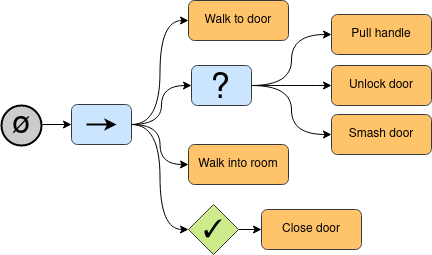
\includegraphics[width=0.6\linewidth]{Images/images/BTTutorial.drawio.png}
\caption{Behavior tree describing the sequence of actions to enter a closed room}
\label{fig:bt_appendix_tutorial}
\end{figure}


